\pdfoutput=1

\documentclass{l4proj}

%
% put any packages here
%

\begin{document}
\title{Abstract Aardvark}
\author{James Stewart}
\date{March 27, 2015}
\maketitle

\begin{abstract}
Abstract Aardvark is an interactive web game designed to provide students with a deeper understanding of inheritance through interactive examples of the "is a" structure. The examples of 
\end{abstract}

\educationalconsent
%
%NOTE: if you include the educationalconsent (above) and your project is graded an A then
%      it may be entered in the CS Hall of Fame
%
\tableofcontents
%==============================================================================

\chapter{Introduction}
\pagenumbering{arabic}
\section{Problem Overview}

The object oriented concept of Inheritance can be a rather confusing subject for the novice programmer. The educational literature(discussed in section \ref{litRev}) backs this assertion through numerous studies showing the ease with which novice programmers can form misconceptions. These misconceptions can be formed due to an ill-conceived linkage between the concept within the paradigm and similar concepts from the real world. They can also be formed from a user's familiarity with another paradigm. These conceptual misunderstandings effect the users comprehension of the inner workings of the programs and leads to less optimal code and less pure object orientation. 

\section{Aims}

The aim of this project is to create an interactive web game to solidify the users understanding of inheritance. The game will then be evaluated to see if it is at all useful for its purpose. As a web application, the game must be usable on a range of devices through a number of commonly used browsers. The game will also aim to provide users varying levels of challenge through carefully designed difficulty mechanism. 

\section{Motivation}

With the ever growing adoption of the object oriented paradigm by industry, it is essentially mandatory for a programmer to have a firm grip on the concepts key to this approach. From the literature available(see section \ref{litRev}) we can see that there are a number of misconceptions students commonly pick up when broaching the topic. This is especially true when it comes to learning the more abstract and complex concepts such as inheritance and polymorphism. As such it is important to provide the learners and educators with appropriate tools to ensure that these misconceptions do not persist moving forward.

Another key motivation is creating a purely conceptual tool with which users can learn about inheritance. The current applications (see section \ref{applications}) designed to help users learn this concepts are , at least for the majority, language specific. This means that the object oriented concepts are introduced whilst tied to a language. Whilst this is common practice for such applications, it can invite the user to develop language specific misconceptions. As such, it is important to provide tools to educators and learners which expose these concepts in their most pure form. 

\section{Outline}

The rest of the report is structured as follows:
\begin{itemize}
\item Chapter \ref{B&R} provides a brief summary of the literature surrounding the approach to teach the object-oriented paradigm as well as short reviews of similar existing applications.
\item Chapter \ref{requirements} contains a list of all of the requirements gathered for the application. 
\item Chapter \ref{design} details the design process of the application and the considerations made during this process. 
\item Chapter \ref{implementation} is dedicated to implementation process and as such covers the mechanisms of each section of the application. 
\item Chapter \ref{evaluation} details the evaluation methods used for the application and contains an analysis and interpretation of the results collected
\item Chapter \ref{c&f} details the areas which have been highlighted for future work and concludes this dissertation. 

\end{itemize}

% \begin{verbatim}

%             > pdflatex example0
%             > bibtex example0
%             > pdflatex example0
%             > pdflatex example0

% \end{verbatim}


\chapter{Background and Research}
\label{B&R}
\section{Literature}
\label{litRev}
Over the last 25 years the object-oriented paradigm has gained widespread adoption in industry. As such there has been an equally widespread adoption in education. Many universities now offer courses on the subject\cite{kentOOP,glasgowOOP,oxfordOOP} and concepts that are cornerstones of the paradigm are now even introduced to students in high-school\cite{sqa}. As with any educational subject, there have been a number of studies into the teaching of the object-oriented paradigm.

\subsection{Approaches to teaching OOP}
\label{approaches}

The computing science educational community seems split on the approach to the introduction and teaching of the object oriented paradigm. There are a number of educators who advocate an `objects first'\cite{empricalOOP} approach to teaching the paradigm. As the name suggests, this approach introduces the learner to objects immediately. This approach generally has the student defining and implementing classes from the beginning focusing on the concrete-creative aspect of programming.   

The second approach taken is that of an `objects later' or when looking at a degree as a whole `procedural first'. `Objects later'\cite{empiricalOOP} is the approach where the students are at first introduced to the data structures and control structures of a language first before introducing them to objects and the more abstract concepts of the paradigm such as encapsulation or inheritance. This approach is highly reflective of the structure that one would usually find in textbooks on object oriented programming. It is of the idea that in order to truly understand the higher level concepts of the paradigm, the student must understand the basic operations of a language. This approach when applied to a degree structure, where a first year covers a procedural language and then in subsequent years studies an object-oriented language can be called `Procedural first'.

Various studies\cite{compOOPComfort,ehlert2007learners,empiricalOOP} have been done to compare the effect of each approach on a students understanding of concepts core to object-oriented paradigm. The paper by Ehlert et al. \cite{empiricalOOP} provided an in-depth empirical analysis of both approaches. It found that although there may be differences in the perceived difficulty of modules between objects first and objects later, that there is no effect to the overall learning gain between the two. From the students perspective it appears that the `objects first' approach is believed to be more difficult\cite{compOOPComfort,ehlert2007learners}. This being said when comparing the perceived difficulty of each method to the difficulty measured via student assessment there appears to be no massive differences in difficulty between each approach. 

There are also papers\cite{programmingInContext,methodologyFirst, 5070749, blowingThingsUp, toolsAndCollections, 6632635} on the tools and pedagogical approaches which can be used to aid the teaching of this paradigm. The most popular approach seems to be that of `methodology first' which is based on the idea that a student should have a strong idea of the concepts and models used by the object-oriented paradigm before they get introduced to the actual languages used and their intricacies. In order to build this mental model the community suggest the use of a visual tool designed to give the learner a deeper understanding of the mechanisms of the paradigm. The gamification of the concepts key to the paradigm have also been attempted by numerous parties. A small review of this can be found later in section \ref{applications}.



\subsection{Difficulties learning inheritance}

Various studies\cite{ehlert2007learners,compOOPComfort,dilatp} have polled teachers and learners on a number of object-oriented concepts to garner their perceived learning difficulty level. Studies by Bilkent et.al and others\cite{compOOPComfort,dilatp} have shown that for inheritance the perceived difficulty of the topic is normal with students finding it neither easy nor hard. This seems to be in direct contradiction to other findings and observations\cite{dilatp,partonomyAndTaxonomy,diffInheritancePolymorphism} such as those found by Ehlert et al.\cite{ehlert2007learners} which ranked inheritance as the 3rd most difficult concept overall. 

An answer for this inconsistant view may have been suggest by Milne et al.\cite{dilatp}, one of the studies which contains views from both learners and teachers. In this study, teachers perceive the difficulty of inheritance to be above average in contradiction to the students view that it is neither difficult nor easy. The paper goes onto discuss the possibility that students perceived difficulty of topics may be due to a lack of proper understanding of the topic leading to a false sense of security for certain conceptually harder topics. 

There are a number of studies\cite{partonomyAndTaxonomy,diffInheritancePolymorphism,taxonomyTaxonomy} which look at inheritance in detail. Teif et al.\cite{partonomyAndTaxonomy} explore the confusion students have between a taxonomy and partonomy. A taxonomy is the model inheritance relationship more commonly referred to as the `is a' relationship and details the hierarchical structure through which objects inherit attributes and methods. A partonomy on the other hand is the idea of possession. A partonomy is a reference to the ownership of an attribute or the `has a' relationship. The paper details the many ways with which these two similar but different relationships can confuse students and the ways which we can avoid this confusion through teaching. 

Liberman et al.\cite{diffInheritancePolymorphism} also look in detail at the misconceptions students can have when looking at inheritance and polymorphism. Altogether they found 60 common misconceptions that students have when covering these topics. Their findings show that there are potential problems which stem from analogies to real world understandings as well as to the operations within other paradigms such as the procedural paradigm. 

\section{Applications}
\label{applications}

This section aims to explore applications within the same domain as AbstractAardvark
\subsection{Java Ninja}
\begin{figure}[h]
    \centering
    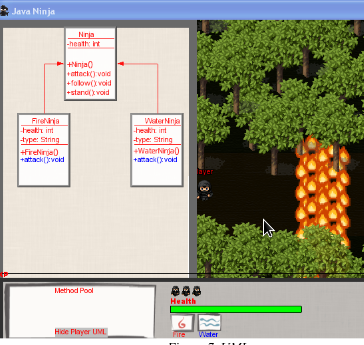
\includegraphics[width=0.35\textwidth]{images/javaNinja}
    \caption{Java Ninja}
    \label{fig:javaNinja}
\end{figure}

Java Ninja(\ref{fig:javaNinja}) is a game developed by researchers\cite{6632635} at Winston-Salem State University and has been designed specifically to teach students the concept of Java inheritance.

The game has the learner play the role of a ninja with powers to create specialised ninjas with specific abilities to tackle the many obstacles within the game. Throughout the game the user comes across multiple obstacles such as fires or type set gates through which only specific ninjas can pass. In order to progress, the user has to create a new subclass of the original ninja class. 

Java ninja is unique in the way that it provides the user with the ability to create subclasses, inherit non-private attributes and methods and override methods without requiring the user to write overly complex code. It also graphically displays relationships between the classes through a sub-window in the UI which displays the relationships in a standard UML format. 

Although this approach is a good one, it shoehorns users into learning the concepts through Java which in itself requires the user to have prior knowledge of the language for use. Abstract aardvark aims to provide the users with a purely conceptual understanding of inhertance without specific ties to a language. 

\subsection{Alice}
\begin{figure}[h]
    \centering
    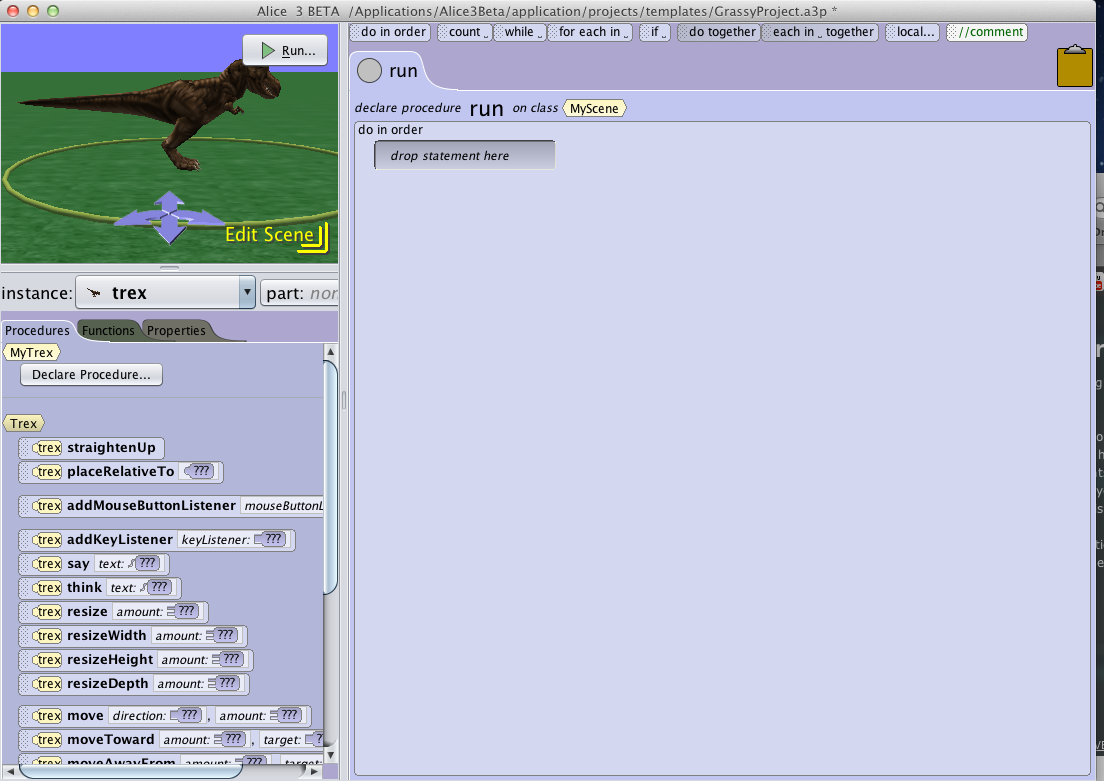
\includegraphics[width=0.35\textwidth]{images/alice}
    \caption{Alice}
    \label{fig:Alice}
\end{figure}
 Alice is a 3d programming environment designed to be a students first interaction with the object oriented programming paradigm. It aims to teach students fundamental programming concepts through the guise of creating 3d environments and movies.
 
Alice makes a decent attempt at visualising the inner processes that occur when you are running your program. It shows exactly what your methods and attributes are through movement animations and area selections of the world and models it uses. 

This being said there are a number of issues with it. Firstly the interface for the IDE is rather difficult to use. When looking for methods or attributes to manipulate your `world' it will often take minutes to find what you are looking for. The tools available for setting up your world are not intuitive and can be rather confusing to a beginner and expert alike.

Alice does allow for class inheritance in its programs but it doesn't make it obvious that it does to it's users. The users can create subclasses of objects by editing preexisting objects, adding new methods to the object at a class level and then saving the object as a new object. Whilst this in a way is inheriting from the previous object class it isn't a true implementation of the concept. 
 
\subsection{BlueJ}
\begin{figure}[h]
    \centering
    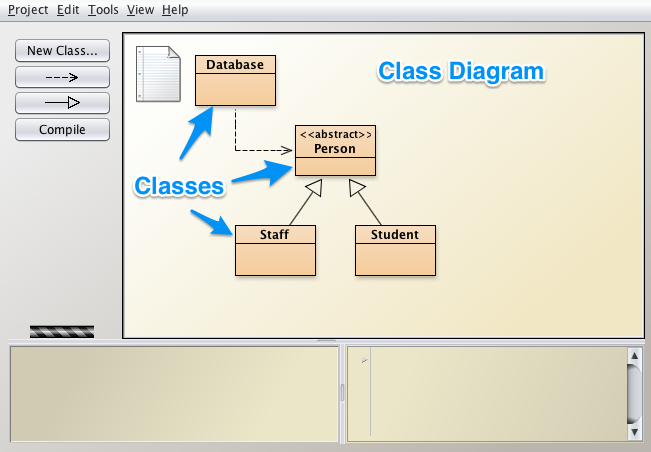
\includegraphics[width=0.35\textwidth]{images/BlueJ}
    \caption{BlueJ}
    \label{fig:BlueJ}
\end{figure}
BlueJ is a graphical IDE designed with the sole purpose of creating Java programs quickly and efficiently.
It was designed with pedagogy in mind and thus has tools which allow you to interact with objects during the coding process. Users can see a number of things through it’s inbuilt graphical tools allowing for a more indepth look at the objects states, attributes and methods. This hopefully helps the understanding of the object oriented concepts which the user should be learning.

One of the major features of blueJ is the class diagram view. This is a graphical view that allows users to develop a class hierrarchy with very little coding. As can be seen in figure \ref{fig:BlueJ} the user is presented with a blueprint like view and can choose to add new classes. They can then create the relationships between classes even going so far as to create abstract classes.

Where BlueJ fails however is it's required knowledge of basic Java. Whilst it may limit the heavy coding required to implement a lot of features it doesn't provide the user with a way to learn about inheritance without being adept enough to go about implementing the class hierrarchy themselves. It therefore acts as a tool to visualise what is going on with their programs solely rather than as a tool to introduce and consolidate the concepts. 



\chapter{Requirements}
\label{requirements}
\section{Gathering Requirements}
\section{Functional Requirements}
\subsection{Must Have}
\subsection{Should Have}
\subsection{Could Have}
\subsection{Would like to have}
\section{Non-Functional Requirements}

\chapter{Design}
\label{design}
\chapter{Implementation}
\label{implementation}
\section{data gathering}
\section{API}
\section{UI}

\chapter{Evaluation}
\label{evaluation}
\chapter{Conclusion and Further Work}
\label{c&f}
%address confusion between taxonomy(is a) and partonomy(has a) 



% %%%%%%%%%%%%%%%%
% %              %
% %  APPENDICES  %
% %              %
% %%%%%%%%%%%%%%%%
% \begin{appendices}

% \chapter{Running the Programs}
% An example of running from the command line is as follows:
% \begin{verbatim}
%       > java MaxClique BBMC1 brock200_1.clq 14400
% \end{verbatim}
% This will apply $BBMC$ with $style = 1$ to the first brock200 DIMACS instance allowing 14400 seconds of cpu time.

% \chapter{Generating Random Graphs}
% \label{sec:randomGraph}
% We generate Erd\'{o}s-R\"{e}nyi random graphs $G(n,p)$ where $n$ is the number of vertices and
% each edge is included in the graph with probability $p$ independent from every other edge. It produces
% a random graph in DIMACS format with vertices numbered 1 to $n$ inclusive. It can be run from the command line as follows to produce 
% a clq file
% \begin{verbatim}
%       > java RandomGraph 100 0.9 > 100-90-00.clq
% \end{verbatim}
% \end{appendices}

%%%%%%%%%%%%%%%%%%%%
%   BIBLIOGRAPHY   %
%%%%%%%%%%%%%%%%%%%%

\bibliographystyle{plain}
\bibliography{bib}

\end{document}
